\documentclass[12pt,a4paper]{article}
\usepackage[utf8]{inputenc}
%\usepackage[slovak]{babel}
\usepackage[IL2]{fontenc}
\usepackage{amsmath}
\usepackage{amsfonts}
\usepackage{amssymb}
\usepackage{graphicx}


%\title{Automatizovaná detekce a klasifikace jevů v časových řadách hydraulických sensorů}
\title{Automatized detection and classification of events in the time series of hydraulic sensors}
\author{Alexander Ma\v{c}ejovsk\'{y} \and \v{S}t\v{e}p\'{a}n Pardubick\'{y}}
\date{\today}

\begin{document}

%%\begin{titlepage}
%%    \centering
%%    \vspace*{2cm}
%%    {\huge\bfseries \maketitle}
%%    \vfill
   % \emph{Last edited on:} \today % Date will update automatically
%%    \vfill
%%\end{titlepage}

\maketitle % Insert title here

\thispagestyle{empty} % Remove page number from title page

\clearpage % Start the table of contents on a new page

\tableofcontents  

\newpage



\section{Introduction}


The domain of sewage management is critical for urban infrastructure, but it is also often overlooked.
The traditional methods of monitoring sewage systems are constrained by the limitations of manual analysis, often resulting in delayed responses to anomalies and missed opportunities for optimization.
Our goal was to create a Python library encapsulating a suite of algorithms, each meticulously designed to address data exploration, anomaly detection, visualization and correction of errors. Leveraging the power of Python's extensive ecosystem of libraries for scientific computing and data analysis, our solution easily integrates into existing workflows, offering a utility for both experts and practitioners in the field. This paper will summarize our work process and display our results to the reader.

\begin{figure}[ht]
  \noindent\makebox[\textwidth]{%
  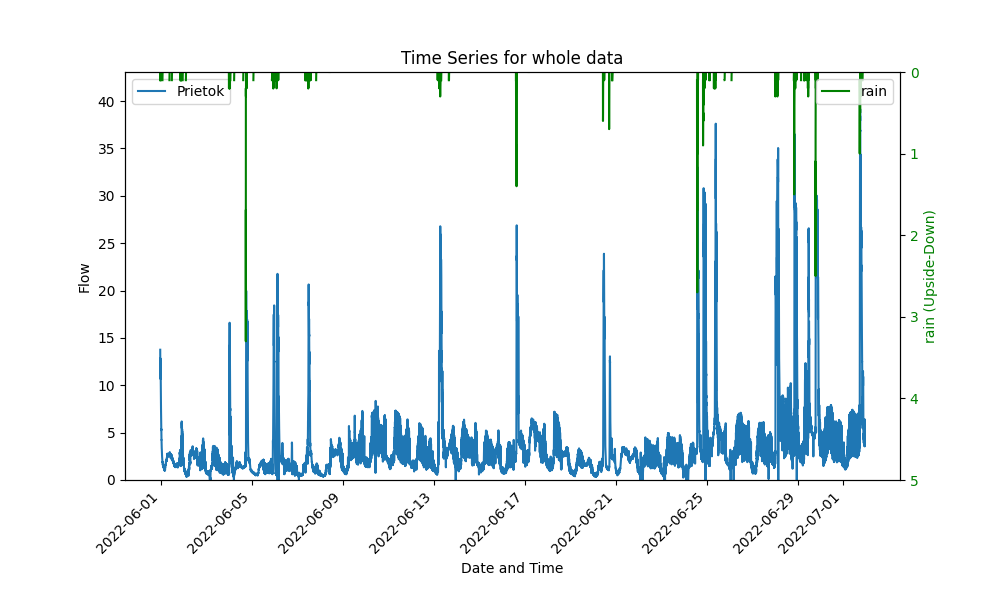
\includegraphics[width=1.4\textwidth]{Rain Dataset.png}}
  \caption{Example of a time series of flow in sewage pipe and measured precipitation. It can be seen that the peeks in the flow coincide with rain.}
    \label{rain_data}
\end{figure}

We were given several time series of flow of water in a sewage system. Each datapoint describes aggregated amount of water that has flown through a fixed control part of a sewer. This amount was calculated from the measured level of the water, it's velocity and the shape of the pipe. This information is gathered by means of various (often pricey) sensors. These sensors can be prone to various types of malfunctions. They can get clogged, displaced or even break. It is important to be able to detect these forms of failures in the time series. The time series of the flow is however very volatile and noisy. It features major upticks in flow coinciding with rain and natural daily cyclicity (peeks and increased volatility in the mornings and evenings when people tend to bathe and use toilet, dishwasher among other causes). Example can be seen in Figure \ref{rain_data}. These fluctuations make it hard to detect malfunctions.

The client wanted us to try and come up with original and unobscured solution to the problem. As such we were given little to information as to how what the errors look like, how to correct them and how to tackle the problem as a whole. Due to neither of us having any expertise in the field of sewage management, our work should be seen as an attempt to creatively explore unknown field and develop new solutions. As such our approach was to creatively utilize standard techniques for working with time series and create a framework for their further utilization, rather than using or developing overly complex methods.


\subsection{Task Description}
Our task can be broken down into the following steps:
\begin{itemize}
  \item Loading and visualizing the data
  \item Performing data exploration
  \item Handle rain and cyclicity
  \item Error definition and identification
  \item Correction of errors
  \item Developing Python library for handling all of these steps
\end{itemize}
There are also several nuances to the assignment, given by the client, that are good to mention here:
\begin{itemize}
    \item While the precipitation data is key for the problem, it cannot be accessed by the methods
    \item Each time series should be viewed in isolation and the data from other time series shouldn't be used
    \begin{itemize}
      \item{We should not fit a big model on all the data and then use it on individual series}
      \item{We cannot utilize any relations between the series (for example to investigate several series in parallel)}
      \item {We aren't given any labels for errors or non-defunct (corrected) series to test the performance}
      \item{While information for both water level and velocity is provided, the time series are to be investigated as univariate - the methods should be developed for flow and then can be later tried on other variables}
    \end{itemize}
\end{itemize}


\section{Data Exploration}
In this section we will focus on exploration and description of the data provided.




\section{Identified Events}




\section{Corrections of Errors}


\section{Performance Evaluation}
no target $\Rightarrow$ not clear how to do this, but detection of events done expertly with the help of consultations,  basic idea for evaluation of corrections could be that no (only few) errors should be detected in already corrected time series 


\section{Python Library}

very brief summary of what the resulting library contains, how it is used, + link to the github page (we should probably restrict it with a password)

Description of utilized python libraries and sources.






\section{Conclusion}





\end{document}